

\section{Kadeishvili's theorem}

One of the main reasons we introduce these $\A$-algebras, instead of just working directly with DG-algebras, is because of a theorem proved by Kadeishvili in \cite{kadeishvili}. We have seen that not all DG-algebras have a quasi-isomorphism to their cohomology algebra---as not all DG-algebras are formal---but this theorem will allow us to sort of approximate the existence of such a morphism. The caveat is that DG-algebras no longer suffice, and we must venture into the world of $\A$-algebras. The idea is to build an $\A$-structure on the cohomology algebra of a DG-algebra, such that instead of a DG-quasi-isomorphism we have an $\A$-quasi-isomorphism connecting them. 

We then want to study these more complicated structures and morphisms in order to figure out if they collapse to our more simple DG-algebra world in certain situations. If we can do and understand this, it will give us a new tool to figure out if a DG-algebra is formal. So far our tool for checking formality of a DG-algebra---namely the Massey products---have been a sort of non-criteria. By this we means that we can use them to easily spot whether a DG-algebra is non-formal, but we can not use them to check formality. This more general theory will allow us to create a more ``perfect'' version of Massey products in order to actually prove that a class of DG-algebras are formal. 

\begin{definition}[Minimal $\A$-algebra]
\label{def:minimal_A_infinity-algebra}
We say an $\A$-algebra $(A, m)$ is minimal if we have $m_1 = 0$. 
\end{definition}

\begin{theorem}[Kadeishvili's theorem]
\label{thm:Kadeishvilis_theorem}
Let $(A,d)$ be a DG-algebra. Then there exists a minimal $\A$-algebra structure on its cohomology algebra $H(A)$, and a quasi-isomorphism of $\A$-algebras $H(A)\rightarrow A$. 
\end{theorem}

Before we look into the proof, we discuss the strategy. We have already seen---at least the beginnings of---how to construct an $\A$-structure from a deformation retraction between a DG-algebra and a chain complex. This is also the idea for this theorem. We construct a particular deformation retract, and use the earlier discussed procedure to produce both the $\A$-structure and the $\A$-quasi-isomorphism that we want. We remind the reader that we are working over a field $k$, so the graded components of the objects are vector spaces, which makes it easy to construct compliments and direct sums. The following construction is due to Lu, Palmieri, Wu and Zhang in \cite{Ext} as a special case of the more general approach by Merkulov in \cite{Merkulov}. 

Let $A=(\bigoplus_{i\in \Z}A^i, d, m)$ be a DG-algebra. As usual we denote $Z^n = \ker d^n$, the $n$-cochains,  and $B^n = \ima d^{n-1}$, the $n$-coboundaries. Since $A$ is in particular a cochain complex we know that $B^n\subseteq Z^n$ is a subspace, i.e. all coboundaries are cocycles. This means that we can find a subspace $H^n$ of $Z^n$ such that $Z^n = B^n\oplus H^n$. Notice that we can identify $H^n(A)\cong H^n$ as we have a split exact sequence
\begin{equation*}
    0\longrightarrow B^n\longrightarrow Z^n\overset{d^n}\longrightarrow H^n(A)\longrightarrow 0 .
\end{equation*}
As $Z^n$ is a subspace of $A^n$ we can also find another subspace $L^n$ such that 
\begin{equation*}
    A^n = Z^n\oplus L^n = B^n\oplus H^n\oplus L^n
\end{equation*}
We can identify $L^n$ with $B^{n+1}$ because of the existence of the split exact sequence 
\begin{equation*}
    0\longrightarrow Z^n\longrightarrow A^n\overset{d^n}\longrightarrow B^{n+1}\longrightarrow 0
\end{equation*}

We can also view the cohomology algebra $H(A)$ as a sub algebra through the identification with $H=\bigoplus_{i\in \Z} H^n$. Denote $i\colon H\longrightarrow A$ the inclusion of $H$ into $A$ and $p\colon A\longrightarrow H$ the projection. Notice that we have $p\circ i = id_H$. The only remaining part---in order to have a deformation retraction---is the homotopy $h\colon A\longrightarrow A$. We will chose this homotopy quite carefully. 

Let us first define some notation. Since $A^n=B^n\oplus H^n\oplus L^n$ we can describe the differential $d$ by nine maps 
\begin{alignat*}{3}
    d^n_{BB}&\colon B^n &&\longrightarrow B^{n+1} \\
    d^n_{BH}&\colon B^n &&\longrightarrow H^{n+1} \\
    d^n_{BL}&\colon B^n &&\longrightarrow L^{n+1} \\
    d^n_{HB}&\colon H^n &&\longrightarrow B^{n+1} \\
    d^n_{HH}&\colon H^n &&\longrightarrow H^{n+1} \\
    d^n_{HL}&\colon H^n &&\longrightarrow L^{n+1} \\
    d^n_{LB}&\colon L^n &&\longrightarrow B^{n+1} \\
    d^n_{LH}&\colon L^n &&\longrightarrow H^{n+1} \\
    d^n_{LL}&\colon L^n &&\longrightarrow L^{n+1} , 
\end{alignat*}
each of them being just the differential projected and restricted to the proper part of the decomposition of $A$. Equivalently they are the parts of the matrix describing the differential, i.e. 
\begin{equation*}
d^n = 
\begin{bmatrix}
    d^n_{BB} & d^n_{BH} & d^n_{BL} \\
    d^n_{HB} & d^n_{HH} & d^n_{HL} \\
    d^n_{LB} & d^n_{LH} & d^n_{LL} 
\end{bmatrix}
\colon B^n\oplus H^n\oplus L^n \longrightarrow B^{n+1}\oplus H^{n+1}\oplus L^{n+1}
\end{equation*}
Because $B^n$ and $H^n$ both consist of cocycles, we know that the differential vanishes on those subspaces. Hence we have 
\begin{equation*}
    d^n_{BB} = d^n_{BH} = d^n_{BL} = d^n_{HB} = d^n_{HH} = d^n_{HL} = 0.
\end{equation*}
We also have no $(n+1)$-coboundaries in $H^{n+1}$ and $L^{n+1}\cong B^{n+2}$, which means we have $d^n_{LH} = d^n_{LL} = 0$ as well.

This means that the matrix for $d^n$ really looks like
\begin{equation*}
d^n = 
\begin{bmatrix}
    0 & 0 & 0 \\
    0 & 0 & 0 \\
    d^n_{LB} & 0 & 0 
\end{bmatrix}    
\end{equation*}

We can now describe the degree $n$ part of our proposed homotopy $h$ as a map 
\begin{equation*}
    h^n\colon B^n\oplus H^n\oplus L^n \longrightarrow B^{n-1}\oplus H^{n-1}\oplus L^{n-1} 
\end{equation*}
given by the matrix 
\begin{equation*}
h^n = 
\begin{bmatrix}
0 & 0 & (d_{LB}^{n-1})^{-1}\\
0 & 0 & 0\\
0 & 0 & 0
\end{bmatrix}
\end{equation*}
Note that this inverse, $(d_{LB}^{n-1})^{-1}$, exists, as we earlier identified the subspace $L^n$ by $L^n \cong B^{n+1}$. 

In order for $h$ to be a homotopy between $id_A$ and $i\circ p$, we need to have 
\begin{equation*}
    id_{A^n} - (i\circ p)^n = d^{n-1}\circ h^{n} + h^{n+1}\circ d^n, 
\end{equation*}
or equivalently stated---that the sum of the maps in the parallelogram in the below diagram, equals the vertical arrow. 
\begin{center}
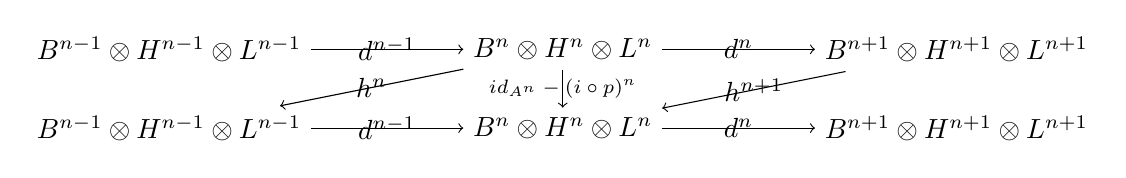
\begin{tikzpicture}
	\node (1) {$B^{n-1}\otimes H^{n-1}\otimes L^{n-1}$};
	\node (2) [node distance=5cm, right of=1] {$B^n\otimes H^n\otimes L^n$};
	\node (3) [node distance=5cm, right of=2] {$B^{n+1}\otimes H^{n+1}\otimes L^{n+1}$};
	
	\node (4) [below of=1]{$B^{n-1}\otimes H^{n-1}\otimes L^{n-1}$};
	\node (5) [node distance=5cm, right of=4] {$B^n\otimes H^n\otimes L^n$};
	\node (6) [node distance=5cm, right of=5] {$B^{n+1}\otimes H^{n+1}\otimes L^{n+1}$};

	\draw [-to] (2) to node [swap]{$h^n$} (4);
	\draw [-to] (3) to node {$h^{n+1}$} (5);
	\draw [-to] (2) to node {{\scriptsize $id_{A^n}-(i\circ p)^n$}} (5);
	
	\draw [-to] (1) to node {$d^{n-1}$} (2);
	\draw [-to] (2) to node {$d^{n}$} (3);
	\draw [-to] (4) to node [swap]{$d^{n-1}$} (5);
	\draw [-to] (5) to node [swap]{$d^{n}$} (6);
\end{tikzpicture}
\end{center}

In matrix notation the left hand side becomes
\begin{equation*}
\begin{bmatrix}
1 & 0 & 0 \\
0 & 1 & 0 \\
0 & 0 & 1
\end{bmatrix}
-
\begin{bmatrix}
0 & 0 & 0 \\
0 & 1 & 0 \\
0 & 0 & 0
\end{bmatrix}
=
\begin{bmatrix}
1 & 0 & 0 \\
0 & 0 & 0 \\
0 & 0 & 1
\end{bmatrix}
\end{equation*}
so we need to confirm that the right hand side is equal to that. We just multiply the matrices we have for the maps, which gives us
\begin{align*}
    d^{n-1}\circ h^n 
    &= 
    \begin{bmatrix}
    0 & 0 & 0 \\
    0 & 0 & 0 \\
    d^{n-1}_{LB} & 0 & 0
    \end{bmatrix}
    \cdot
    \begin{bmatrix}
    0 & 0 & (d_{LB}^{n-1})^{-1}\\
    0 & 0 & 0\\
    0 & 0 & 0
    \end{bmatrix} \\
    &= 
    \begin{bmatrix}
    0 & 0 & 0 \\
    0 & 0 & 0 \\
    0 & 0 & d^{n-1}_{LB}(d_{LB}^{n-1})^{-1} 
    \end{bmatrix} \\
    &= 
    \begin{bmatrix}
    0 & 0 & 0 \\
    0 & 0 & 0 \\
    0 & 0 & 1 
    \end{bmatrix}
\end{align*}
and
\begin{align*}
    h^{n+1}\circ d^n 
    &=
    \begin{bmatrix}
    0 & 0 & (d_{LB}^{n})^{-1}\\
    0 & 0 & 0\\
    0 & 0 & 0
    \end{bmatrix}
    \cdot 
    \begin{bmatrix}
    0 & 0 & 0 \\
    0 & 0 & 0 \\
    d^{n}_{LB} & 0 & 0
    \end{bmatrix} \\
    &=
    \begin{bmatrix}
    (d_{LB}^{n})^{-1}d^{n}_{LB} & 0 & 0\\
    0 & 0 & 0\\
    0 & 0 & 0
    \end{bmatrix} \\
    &=
    \begin{bmatrix}
    1 & 0 & 0\\
    0 & 0 & 0\\
    0 & 0 & 0
    \end{bmatrix} .
\end{align*}
Hence we have
\begin{align*}
    h^{n+1}\circ d^n + d^{n-1}\circ h^n 
    &= 
    \begin{bmatrix}
    0 & 0 & 0 \\
    0 & 0 & 0 \\
    0 & 0 & 1 
    \end{bmatrix}
    + 
    \begin{bmatrix}
    1 & 0 & 0 \\
    0 & 0 & 0 \\
    0 & 0 & 0 
    \end{bmatrix} \\
    &= 
    \begin{bmatrix}
    1 & 0 & 0 \\
    0 & 0 & 0 \\
    0 & 0 & 1
    \end{bmatrix} \\
    &= 
    id_{A^n} - (i\circ p)^n , 
\end{align*}
which shows that $h$ is in fact a chain homotopy between $id_A$ and $i\circ p$. This means that we finally have our deformation retraction
\begin{center}
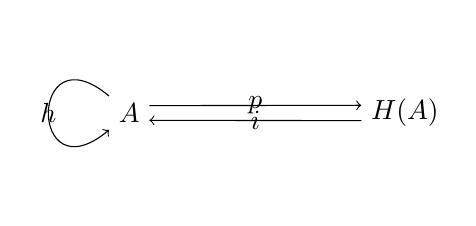
\begin{tikzpicture}
	\node (1) {$A$};
	\node (2) [node distance=3.5cm, right of=1] {$H(A)$};
	
	\draw [to-, out=220, in=140, loop] (1) to node {$h$} (1);
	\draw [-to] (1.20) to node {$p$} (2.170);
	\draw [-to] (2.190) to node {$i$} (1.340); . 
\end{tikzpicture}
\end{center}

Note that this deformation retraction is not unique, as it requires making choices for the subspaces $H^n$ and $L^n$. Thus we can get many different such deformation retractions by altering these choices. In the theorem we want to prove, namely that such a deformation retraction gives us an $\A$-structure on the cohomology algebra, we will get different, albeit $\A$-quasi-isomorphic $\A$-structures when we alter the choices of the subspaces. Since we are only interested in an $\A$-structure on $H(A)$ such that it is $\A$-quasi-isomorphic to $A$, these choices of subspaces are not important---as we have our desired $\A$-quasi-isomorphism regardless. This is because we are not really interested in the structure itself, merely its existence, and its relation to formality. 

We now restate Kadeishvili's theorem in this new situation we have created.

\begin{theorem}[Kadeishvili's theorem]
\label{thm:Kadeishvilis_theorem2}
Let $(A, m, d)$ be a DG-algebra and $(A, H(A), p, i, h)$ be the deformation retraction onto its cohomology algebra described above. Then there is a minimal $\A$-structure $\{m_n\}$ on $H(A)$ and an $\A$-quasi-isomorphism $I\colon H(A)\longrightarrow A$ that extends $i$. 
\end{theorem}
\begin{proof}
We let $m_1=0$, $I_1=i$ and $h\lambda_1 = -id_A$. Then for $n\geq 2$ we recursively define
\begin{equation*}
    \lambda_n = \sum_{k=1}^{n-1}(-1)^{k+1}m(h\lambda_k\otimes h\lambda_{n-k})
\end{equation*}
Then our $\A$-structure and $\A$-quasi-isomorphism is given by 
\begin{align*}
    m_n &= p\circ \lambda_n \\
    I_n &= h\circ \lambda_n
\end{align*}
\end{proof}

We call such a minimal $\A$-structure on the cohomology algebra $H(A)$---coming from a deformation retraction of the type above---a Merkulov model of $A$. 

We will not prove that these do in fact satisfy the Stasheff identities, but we refer the reader to \cite{kadeishvili} for the original, and much more general proof. We do however write out what happens for some low $n$. 

% \begin{proof}
% Recall that the deformation retraction comes from a splitting $A=B\oplus H\oplus L$, where $B^n = \ima d^{n-1}$ and $H\cong H(A)$. For any $b\in B$ there is a unique $l\in L$ such that $b = d(l)$. We then define a map $Q\colon B\longrightarrow L$ such that $Q(b)=l$. We then get that $Qd = id_B$ and $dQ = id_L$.

% For any $[a] \in H(A)$ there is a unique $a_0\in H$, representing the cohomology class $[a]$. We define $I_1([a])=a_0$ and $I_2 = Q(I_1 m_2 - m(I_1\otimes I_1))$, where $m$ is the product in $A$, and $m_2$ is the induced product in $H(A)$. Here on we use an inductive argument. Suppose that $m_j$ and $I_j$ have been defined for $1< k$. 

% Let $F_k$ be the map defined by 
% \begin{equation*}
%     F_k = \sum_{i+j = k}(-1)^{i-1}m(I_i\otimes I_j) - \sum_{r+s+t=k}(-1)^{r+st}I_{r+1+t}(id^{\otimes r}\otimes m_s\otimes id^{\otimes t}).
% \end{equation*}
% Notice that it only uses already defined $I_i$'s and $m_i$'s, so it is in fact a well defined map. 

% The relation we need then becomes 
% \begin{equation*}
%     d I_k = I_1 m_k - F_k.
% \end{equation*}
% As we have that $\partial F_k = 0$ we know that every time we use it on an element $x_1\otimes \cdots \otimes x_k \in H(A)^{\otimes k}$ we get a cocycle in $A$. We then define $m_k$ to be the map that takes in such an element $x_1\otimes \cdots \otimes x_k$ and returns the cohomology class of the cycle that $F_k$ produces. More simply we can write that $m_k = \overline{F_k}$, i.e. the induced map on cohomology. Since $I_1$ chooses cocycles for the cohomology classes we get that $I_1m_k-F_k$ is cohomologous to zero. For some free generators $x_i \in H(A)$ we can then define $I_k$ to be a map that sends the product of such free generators $x_1\otimes \cdots \otimes x_k$ to a cocycle bounding $(I_1 m_k-F_k)(x_1\otimes \cdots \otimes x_k)$. The whole map is defined by extending this linearly. 

% %We then define $m_k$ and $I_k$ from the relations $I_1 m_k - d I_k = F_k$ and $I_k = Q(I_1 m_k - F_k)$. 
% \end{proof}
% \todo[inline]{Can we check the relevant calculations to check that this in fact gives an $\A$-structure?}

For $n=2$ we get
\begin{equation*}
    m_2 = p\circ \lambda_2 = p(m(h\lambda_1)\otimes h\lambda_1) = p(m(-id_A\otimes -id_A) = pm
\end{equation*}

which is just the induced multiplication from $A$ on $H(A)$. Earlier when we looked at transferring algebraic structures, we also used the map $i$ to describe the induced operation, but here we omit it, as we think of $H^i$ as a subspace of $A^i$. For $n=3$ we get 
\begin{align*}
    m_3 
    &= p\circ \lambda_3 \\
    &= p(m(h\lambda_1\otimes h\lambda_2)-m(h\lambda_2\otimes h\lambda_1)) \\
    &= p(m((-id_A)\otimes hm)-m(hm\otimes (-id_A))) \\
    &= p(m(hm\otimes id_A)-m(id_A\otimes hm))
\end{align*}
which we should recognize as the same $m_3$ we constructed from the general deformation retraction we studied earlier, namely the associating homotopy between $m_2(id\otimes m_2)$ and $m_2(m_2\otimes id)$. Since $m_2$ is just the induced product on $H$, we actually know that it is associative, i.e. $m_2(id\otimes m_2)-m_2(m_2\otimes id)=0$, as it is isomorphic to $H(A)$, which is an associative DG-algebra. If we look at the $n=3$ equation defining an $\A$-algebra we have 
\begin{equation*}
    m_2(id\otimes m_2)-m_2(m_2\otimes id) = m_1 m_3 + m_3(m_1\otimes id\otimes id + id\otimes m_1\otimes id + id\otimes id \otimes m_1), 
\end{equation*}
but, as we have $m_1=0$, we are totally fine with having an associative product in this scenario! This means that we have $\partial m_3 = 0$, i.e. that it is a cocycle in $Hom(A^{\otimes 3}, A)$. This, however, does not mean it zero itself.

We mentioned earlier that an alternative way of describing the Stasheff identities was given by 
\begin{equation*}
    \partial m_n = - \sum_{r+s+t=n}(-1)^{r+st}m_{r+s+t}(id^{\otimes r}\otimes m_s\otimes id^{\otimes t})
\end{equation*}
where $r,s,t\geq 1$ and $\partial m_n = m_1m_n - (-1)^{|m_n|}m_n\left(\sum_{r=0}^{n-1}(id^{\otimes r}\otimes m_1\otimes id^{\otimes n-r-1})\right)$. Since all of the terms in $\partial m_n$ contain a copy of $m_1$, we know that the entire sum will be zero, i.e. $\partial m_n = 0$, meaning that all the higher operations are cocycles in their respective cochain complexes $Hom(A^{\otimes n}, A)$. Hence the Stasheff identities for the $\A$-structure we get from Kadeishvili's theorem are
\begin{equation*}
    \sum_{r+s+t=n}(-1)^{r+st}m_{r+s+t}(id^{\otimes r}\otimes m_s\otimes id^{\otimes t}) = 0
\end{equation*}
for $r, s, t\geq 1$. We earlier formed an upside down triangle of trees representing these Stasheff identities. If we remove the top and bottom row of this triangle we are left with the relation just described. Notice that this new truncated upside down triangle contains 
\begin{equation*}
    \left(\sum_{i=1}^n i\right) - n-1 = \left(\sum_{i=1}^{n-1} i\right) -1
\end{equation*}
trees, i.e. one less than the $n-1$'st triangle number. This is not by coincidence equal to the number of facets in $K(n+1)$, the $n+1$'st Stasheff associahedron. 



\begin{remark}
There are several generalizations of Kadeishvili's theorem. Kadeishvili's original proof holds over general commutative rings, if one requires that the cohomology algebra $H(A)$ is a projective module over $A$. This result was extended in \cite{Sagave} to hold for any commutative ring, without any assumptions for $H(A)$---if one instead of a minimal $\A$-algebra uses so-called minimal derived $\A$-algebra. The theorem was later shown to hold if $A$ is an $\A$-algebra instead of just a DG-algebra. See \cite{transfer} for explicit formulas and proofs. This means that the transfer of an $\A$-algebra through a deformation retraction, is again an $\A$-algebra.

The results have also been generalized to the theory of $\infty$-operads, where such a transfer is possible for several other types of algebras, notably DG-Lie-algebras. Most of these results are contained in \cite{operads}. Note that in these other settings the theorem is often referred to as ``the homotopy transfer theorem'' or the ``minimal models theorem''. 
\end{remark}






\subsection{Connection to formality}

Now that we have this more general approach to studying the relationship between a DG-algebra and its cohomology algebra, we need to know how it relates back to our original interests---namely formality. Recall that by \cref{thm:span}, $A$ being a formal DG-algebra means that we have a span of DG-quasi-isomorphisms between $A$ and $H(A)$, i.e. $H(A)\longleftarrow M\longrightarrow A$. By Kadeishvili's theorem we now have more than a DG-structure on $H(A)$, as we have in fact an $\A$-structure $\{m_n\}$, but we also have a direct $\A$-quasi-isomorphism $q\colon H(A)\longrightarrow A$. We know that if $m_n = 0$ for $n\geq 3$ then $H(A)$ is in fact a DG-algebra, so we can think of these possibly non-trivial $m_n$'s as measuring how far away $A$ is from being formal. This is of course informal, but it will soon turn out to also be a precise statement. 

One of the other main reasons for passing to $\A$-algebras is that their homotopy theory is better behaved than for DG-algebras. We have in fact already seen this, as a complex homotopy equivalent to a DG-algebra is not necessarily a DG-algebra, but by the generalizaton of Kadeishvili's theorem we mentioned, this property in fact holds for $\A$-algebras. This means that being an $\A$-algebra is a ``homotopy stable'' property. 

We have also seen that DG-quasi-isomorphisms are not the nicest ones, as they are not homotopy invertible. This is because not all isomorphisms in the homotopy category $hoDGA_k$ comes from a DG-quasi-isomorphism in $DGA_k$. This resulted is us having to use zig-zags and spans of DG-quasi-isomorphisms instead of just direct ones. This property is luckily also fixed by passing to $\A$-algebras, meaning that all $\A$-quasi-isomorphisms are $\A$-homotopy equivalences. 


\begin{definition}[$\A$-homotopy]
\label{def:A_infinity-homotopy}
Let $(A, m^A)$ and $(B, m^B)$ be $\A$-algebras. Two $\A$-morphisms $\{f_n\}, \{g_n\}$ between them are called homotopic if there exists a family of graded homogeneous multilinear degree $-1$ maps $h_n:A^{\otimes n}\longrightarrow B$, such that 
\begin{equation*}
    g_n-f_n = \sum_{i_1+\cdots i_r = n}m^B_{r+1+t} (g_{i_1}\otimes \cdots g_{i_t}\otimes h_s \otimes f_{i_{t+1}}\otimes \cdots \otimes f_{i_r} ) + \sum_{r+s+t = n}h_{r+1+t} (id^{\otimes r}\otimes m^A_s \otimes id^{\otimes t})
\end{equation*}
where $r, t\geq 0, n, s\geq 1$ as usual. 
\end{definition}


\begin{proposition}
\label{prop:infty-qi_homotopy_invertible}
Let $(A, m^A)$ and $(B, m^B)$ be $\A$-algebras and $q:A\rightarrow B$ an $\A$-quasi-isomorphism. Then there exists an $\A$-quasi-isomorphism $q':B\rightarrow A$ that is a $\A$-homotopy inverse of $f$. This means that the class of $\A$-quasi-isomorphisms is the same as the class of $\A$-homotopy equivalences. 
\end{proposition}

We wont prove this result, as the proof uses some machinery that we will not cover in this thesis. More precisely one at least needs the bar and cobar constructions for $\A$-algebras. The reader interested in the proof is referred to \cite[Corollary 1.3.1.3]{french1}. 

The next step is to figure out how an $\A$-quasi-isomorphism relates to a DG-quasi-isomorphism. This is done through the following result.

\begin{corollary}
\label{cor:zigzag-quasi}
Two DG algebras $(A, d_A)$ and $(B, d_B)$ is connected by a zig-zag of quasi-isomorphisms
\begin{equation*}
    A \overset{\sim}\longleftarrow \bullet \overset{\sim}\longrightarrow \cdots \overset{\sim}\longleftarrow \bullet \overset{\sim}\longrightarrow B, 
\end{equation*}
i.e. they are quasi-isomorphic, if and only if there is an $\A$-quasi-isomorphism $A\rightarrow B$. 
\end{corollary}

\begin{proof}
Assume we have a zig-zag of DG-quasi-isomorphisms between $A$ and $B$. Recall that by \cref{thm:span} we can reduce the zig-zag to a single span of DG-quasi-isomorphisms $A\overset{q}\longleftarrow C\overset{p}\longrightarrow B$. We now interpret $A$, $B$ and $C$ as $\A$-algebras, and $q, p$ as morphisms of $\A$ algebras. This is the same standard procedure we have described before, i.e. letting $m^A_n = m^B_n = m^C_n = 0$ for all $n\geq 3$ and defining $\{q_n\}$ by $q_1 = q$ and $q_m = 0$ for $m\geq 2$ and similarly for $p$. By abuse of notation we denote these $\A$-morphisms again by $q$ and $p$. Notice that since $q$ and $p$ are DG-quasi-isomorphisms, then $q$ and $p$ are $\A$-quasi-isomorphisms as well. We then have a span $A\overset{q}\longleftarrow C \overset{p}\longrightarrow B$ of $\A$-quasi-isomorphisms. By \cref{prop:infty-qi_homotopy_invertible} we know these are invertible up to homotopy, hence we have an $A$-quasi-isomorphism $q'\colon A\longrightarrow C$ such that $q\circ q' \sim id_A$ and $q'\circ q \sim id_C$. 

Since composition of two $DG$-quasi-isomorphisms is again a DG-quasi-isomorphism we know that this is the case for composition of $\A$-quasi-isomorphisms as well, as it only depends on the arity $1$ map. Thus $q'\circ p$ is an $\A$-quasi-isomorphism from $A$ to $B$. Notice that this can no longer have $(q'\circ p)_m = 0$ for $m\geq 2$ in general, as that would contradict DG-quasi-isomorphism being homotopy invertible. 

The other direction also holds, but to construct the zig-zag from a $\A$-quasi-isomorphism we again need the previously mentioned bar and cobar construction. To outline the idea, we can produce a DG-algebra $U(A)$ through the bar and cobar construction from an $\A$-algebra $A$. This can be though of as an ``anti Merkulov model''. This DG-algebra is universal, in the sense that any $\A$-morphism from $A$ to a DG-algebra $B$ factorizes uniquely through $U(A)$. Moreover $U(A)$ is $\A$-quasi-isomorphic to $A$. It can then be shown that if $A$ is a DG-algebra, then the map $U(A)\longrightarrow A$ is a DG-quasi-isomorphism. 

In our case we have two DG-algebras $A$ and $B$ and a $\A$-quasi-isomorphism $q\colon A\longrightarrow B$. We then get a zig-zag
\begin{equation*}
    A\overset{q_A}\longleftarrow U(A) \overset{U(q)}\longrightarrow U(B)\overset{q_B}\longrightarrow B
\end{equation*}
where $U(q)$ is a DG-quasi-isomorphism when $q$ is an $\A$-quasi-isomorphism. Hence we have our wanted zig-zag of DG-quasi-isomorphisms. 
\end{proof}

These results allow us to characterize formal DG-algebras by use of $\A$-morphisms instead of zig-zags of DG-morphisms. 


\begin{corollary}
\label{cor:formal_A_infinity-qi}
Let $(A, d_A)$ be a DG-algebra and $H(A)$ its cohomology algebra, treated as a DG-algebra with trivial differential. Then $A$ is formal if and only if there is an $\A$-quasi-isomorphism $q\colon H(A)\longrightarrow A$. 
\end{corollary}

Notice here that this is not the same statement as Kadeishvili's theorem, as here $H(A)$ is purely a DG-algebra, and not endowed with an $\A$-structure. We can however restate the corollary in more similar terms to Kadeishvili's theorem, then saying that a DG-algebra is formal if and only if its Merkulov model is again a DG-algebra, i.e. it has $m_i=0$ for all $i\geq 3$. 





